\section{Metodologia}

% TABELA DE MATERIAIS
\begin{table}[h]
\centering
\caption{Materiais utilizados.}
\begin{tabular}{ll}
\toprule\midrule
Material & Qntd. \\
\midrule
Aparato de Millikan & 1 \\
Fonte de tensão variável (0-600 V, DC) & 1 \\
FlexCam básica & 1 \\
Chave comutadora & 1 \\
Base tripé & 1 \\
Voltímetro & 1 \\
Mangueira  & 1 \\
Cabos de conexão (32 A) & 10 \\
\midrule\bottomrule
\end{tabular}
\label{tab: materiais}
\end{table}

O aparato foi montado conforme a Fig. \ref{fig: aparato}. 
Os materiais utilizados são mostrados na Tab. \ref{tab: materiais}.
O aparato de Millikan consiste em uma pera insufladora que borrifa óleo no espaço entre as placas de um capacitor.
Esse espaço é fechado para o ambiente externo, e e possui iluminação própria.
Há um microscópio que permite observar as gotículas dentro do aparato. 
Uma câmera de haste flexível foi posicionada na lente ocular do microsćopio, e o sinal era transmitido para uma tela maior, 
de modo que era possível facilmente observar o movimento das gotículas.
Dentro do aparato, há um micrômetro ocular, com 30 divisões equivalentdo a 0,89 mm.
A ligação entre o capacitor e a fonte foi feita através de uma chave comutadora, de modo que era possível 
inverter a polaridade no capacitor, e assim inverter o sentido do campo elétrico.
Em paralelo à chave, foi conectado um voltímetro. 

% FOTO DO APARATO EXPERIMENTAL
\begin{figure}[h]
\centering
\caption{Aparato experimental do experimento de Millikan.}
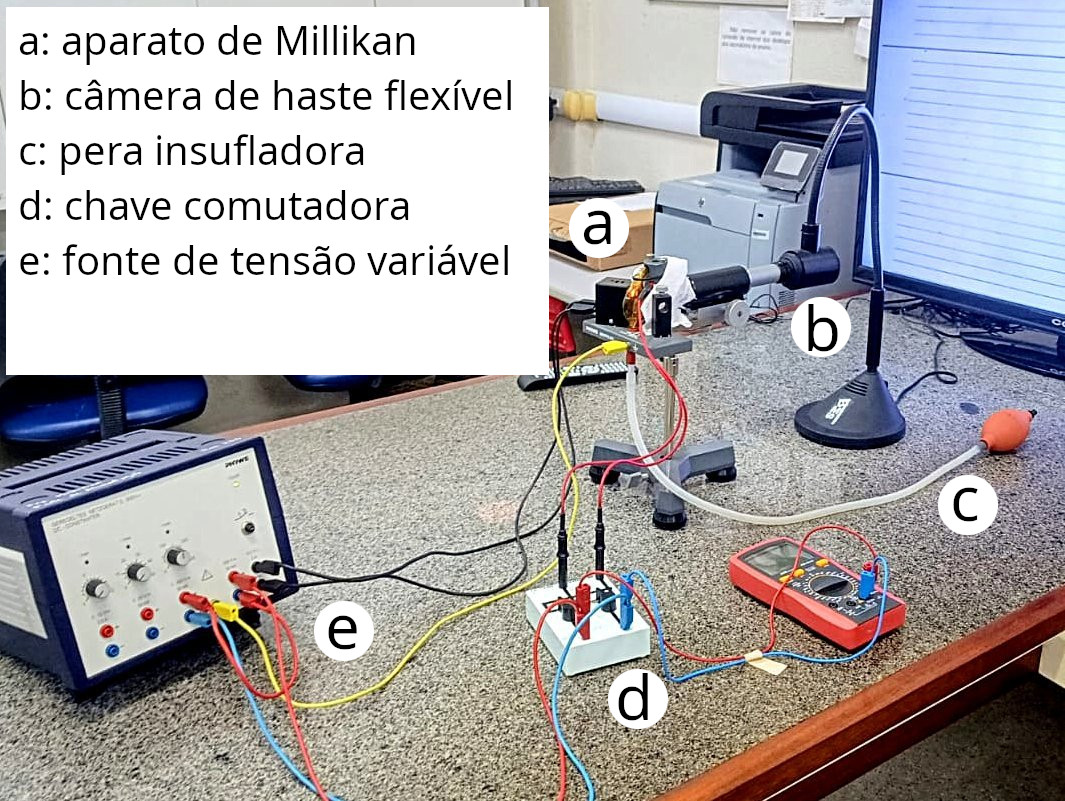
\includegraphics[width = .8\linewidth]{imagens/aparato.jpeg}
\small{\\Fonte: Autor, 2026.}
\label{fig: aparato}
\end{figure}
Primeiramente, foram borrifadas	 gotas de óleo de silicone utilizando a pera insufladora. 
Durante o trajeto, uma determinada gota tem chance de sofrer eletrização por atrito, adquirindo assim uma pequena carga. 
Enquanto as gotas eram observadas na tela, a polaridade no capacitor era invertida, de modo que uma gota 
devidamente eletrizada inverteria seu sentido de movimento. 
Após encontrar uma gota desse tipo, a chave era alternada diversas vezes, enquanto o movimento de subir e descer da gota
era observado.

Enquanto isso, a tela estava sendo gravada com um aparelho celular. 
O vídeo foi analizado posteriormente e foram coletados diversos pares $(t_s, t_d)$, onde $t_s$ é o tempo que leva para 
uma determinada gota percorrer 10 divisões do micrômetro subindo, e $t_d$ é o tempo que a mesma gota leva para percorrer 
as mesmas 10 divisões descendo. Dividindo a distância $(10\text{ div})\times(0,89\text{ mm} / 1 \text{ div}) = 2,967 \times 10^{-5} \text{ m}$ pelos pares de tempos, foi possível obter os pares $(v_s, v_d)$. 
Utilizando então as eqs. \eqref{eq: r} e \eqref{eq: q'}, foi possível obter os valores de $q$ e $r$ para cada gota. Foram realizadas medidas para diferentes valores de tensão.

Para haver consistência com as hipóteses feitas, tomou-se o cuidado de não escolher gotas em que $v_s$ e $v_d$ diferissem de mais de 30$\%$, e nem gotas que apresentassem movimento aparentemente acelerado.  

Utilizando os dados da Tab. \ref{tab: grandezas}, foi possível calcular os valor da constante $A$ que aparece nas eq. \eqref{eq: r} como sendo $A = \qty{6,406e-5}{\meter\tothe{1/2}\second\tothe{1/2}}$.

% TABELA DE GRANDEZAS
\begin{table}[h]
\centering
\caption{Grandezas conhecidas.}
\begin{tabular}{ll}
\toprule\midrule
Grandeza &  Valor \\
\midrule
Separação das placas do capacitor & $d =\qty{2,5e-3}{\meter}$ \\
Densidade do óleo de silicone & $\sigma=\qty{1,03e3}{\kilo\gram\per\meter\tothe 3}$ \\
Densidade do ar & $\rho=\qty{1,293}{\kilo\gram\per\meter\tothe3}$ \\
Viscosidade do ar & $\eta=\qty{1,82e-5}{\kilo\gram\per\meter\per\second}$ \\
Aceleração da gravidade & $g=\qty{9,81}{\meter\per\second\tothe 2}$ \\
\midrule\bottomrule
\end{tabular}
\label{tab: grandezas}
\end{table}

